% This is samplepaper.tex, a sample chapter demonstrating the
% LLNCS macro package for Springer Computer Science proceedings;
% Version 2.21 of 2022/01/12
%
\documentclass[runningheads]{llncs}
%
% \pdfminorversion=4

\usepackage[T1]{fontenc}
\usepackage{microtype}
\usepackage{graphicx}
\usepackage{multirow}
\usepackage{color}
\begin{document}

\title{Data Augmentation for EEG Motor Imagery Classification using Diffusion Model}
\titlerunning{EEG Augmentation with Diffusion Model}
\author{Nutapol Soingern\inst{1} \and
Akraradet Sinsamersuk\inst{1} \and
Chaklam Silpasuwanchai\inst{1}}
\authorrunning{Nutapol et al.}
% \author{Nutapol Soingern$^1$,Akraradet Sinsamersuk$^2$,Chaklam Silpasuwanchai$^3$}

\institute{Asian Institute of Technology, School of Engineering and Technology, Data Science and Artificial Intelligence, Pathum Thani, Thailand
\email{nutapol1997@gmail.com}\\
\email{akraradets@gmail.com}\\
\email{chaklam@ait.asia}\\
}

\maketitle

% \address{Asian Institute of Technology, School of Engineering and Technology, Data Science and Artificial Intelligence, Pathum Thani, Thailand}
% \ead{nutapol1997@gmail.com, akraradets@gmail.com, chaklam@ait.asia}
% \vspace{10pt}
% \begin{indented}
% \item[]November 2023
% \end{indented}

\begin{abstract}
\sloppy
Motor imagery classification using electroencephalogram (EEG) signals is an important research topic that has been extensively studied in the field of brain-computer interfaces (BCIs). 
However, due to the limited amount of available data, the possibility of overfitting is a challenge, especially when using a deep-learning classifier. 
One way to address this is by performing data augmentation. 
This paper investigates the efficacy of the diffusion model as a data augmentation method for motor imagery classification. 
We evaluated the diffusion method by comparing it with commonly-used EEG data augmentation techniques namely such as Noise Addition, Fourier Transform Surrogates, Frequency Shift, and SmoothTimeMask. 
The result shows that the diffusion method outperformed other methods in terms of classification accuracy by 17.49\%. 
The Kullback-Leibler (KL) divergence is used for assessing the similarity between the training set (with and without augmentation) and validation set, thus showing the effectiveness of the diffusion approach compared to other techniques.
\end{abstract}
\keywords{Motor Imagery \and EEG \and Brain Computer Interface \and Deep Learning \and Data Augmentation \and Diffusion \and KL divergence}

%
% Uncomment for keywords
% \vspace{2pc}
% \noindent{\it Keywords}: Motor Imagery, EEG, Brain Computer Interface, Deep Learning, Data Augmentation, Diffusion, KL divergence
%
%
% Uncomment for Submitted to journal title message
%\submitto{\JPA}
%
% Uncomment if a separate title page is required
%\maketitle
% 
% For two-column output uncomment the next line and choose [10pt] rather than [12pt] in the \documentclass declaration
%\ioptwocol
%
\section{Introduction}

Brain-computer interfaces (BCI) establish a direct pathway between the human brain and a computer via signal processing and decoding techniques. 
One classic paradigm of EEG is motor imagery (MI), in which its physiological basis is based on body movements or imagined movements that can produce $\alpha$ (8-13 Hz) and $\beta$ (13-30 Hz) event-related synchronization (ERS) and event-related desynchronization (ERD) rhythms in the motor-sensory areas of the brain \cite{wolpaw2013brain}. 
Recently, the deep learning (DL) model has been used for motor imagery classification. 
For example, EEGNet \cite{lawhern2018eegnet} is a compact convolutional neural network designed for EEG-based brain-computer interfaces that effectively extracts spatial-temporal features from EEG signals.
In any case, the paucity of data is a prevalent issue in the field of EEG classification, as it hinders the development and performance of DL models.
Consequently, a common symptom is overfitting, which reduces the model's accuracy and robustness on test set \cite{bilbao2017overfitting}. 

Data augmentation (DA) has been widely used to improve the robustness and accuracy of DL by artificially increasing the number of training data.
Traditional EEG data augmentation methods include \texttt{Noise Addition} \cite{wang2018data,parvan2019transfer,li2019channel}, fourier transform surrogates \cite{schwabedal2018addressing}, \texttt{Frequency Shift}ing \cite{rommel2021cadda,rommel2022data} and \texttt{\texttt{SmoothTimeMask}} \cite{mohsenvand2020contrastive}.
\texttt{Noise Addition} \cite{li2019channel,parvan2019transfer} adds random white noise to all channels.
Fourier transform surrogates \cite{schwabedal2018addressing} randomizes the Fourier-transform (FT) phases of temporal-spatial data and generates surrogates that approximate examples from the data-generating distribution. \texttt{Frequency Shift}ing \cite{rommel2021cadda,rommel2022data} randomly shifts the frequency spectrum on all channels.
Last, \texttt{\texttt{SmoothTimeMask}} \cite{mohsenvand2020contrastive} randomly masks consecutive time steps of the EEG signal and replaces them with zeros, in which the motivation is to force the model to disregard minor irrelevant events.

Recently, diffusion model \cite{ho2020denoising} was proposed which generates synthetic data based on Langevin dynamics.
These models naturally admitted a progressive lossy decompression scheme.
Diffusion mode has been used as a DA method to generate synthetic training data for skin disease classification \cite{akrout2023diffusion}, prostate cancer detection \cite{hao2021comprehensive}, chest X-ray imaging \cite{motamed2021data}, etc.

In this work, we demonstrated the use of the diffusion model for data augmentation.
Particularly, we developed our diffusion model based on \texttt{WaveGrad} \cite{chen2020wavegrad} as a DA method for motor imagery classification.
\texttt{WaveGrad} has been initially for audio waveform generation.
The proposed approach involves utilizing score matching \cite{song2020sliced, song2020improved} and diffusion probabilistic \cite{sohl2015deep, ho2020denoising} models to estimate gradients of the data density within a conditional model. 
Because \texttt{WaveGrad} is shown to be successful in waveform generation, we apply the technique in the EEG signal with sequence length adjusted.
The process involves initializing the model with a Gaussian white noise signal and subsequently improving the signal quality through an iterative process that utilizes a gradient-based sampler that is conditioned on the mel-spectrogram.
We evaluated the effect of the proposed method by performing DA on BCI Competition IV 2a \cite{brunner2008bci} with various sizes of synthetic data with five standards EEG MI models (EEGNet \cite{lawhern2018eegnet}, ATCNet \cite{altaheri2022physics}, EEG-ITNet \cite{salami2022eeg}, Deep ConvNet \cite{schirrmeister2017deep} and ShallowFBCSPNet \cite{schirrmeister2017deep}). 
The proposed method improves the performance of classification models and outperforms other traditional EEG data augmentation methods. 



\section{Related Work}
We reviewed commonly-used data augmentation for EEG MI such as \texttt{Noise Addition}, \texttt{Fourier Transform Surrogates}, \texttt{Frequency Shift} and \texttt{SmoothTimeMask}.

\subsection{Noise Addition}
\texttt{Noise Addition} has two main categories for adding noise to the EEG signals for DA \cite{lashgari2020data}.
The first category regards adding various types of noise, such as Gaussian noise, Poisson noise, salt-and-pepper noise, etc., each of which has its own set of parameters (such as mean and standard deviation), to the original signal.
The second category converts EEG signals to image sequences and then adds noise to the resulting image sequences. 
In any case, the introduction of noise to the training data is assumed to enhance the robustness of the model by compelling it to learn features that were less susceptible to minor fluctuations in the data.
Indeed, such simulation of EEG data variability was commonly utilized to replicate the effects of electrode noise or subject movement during experimental procedures.
Previous research has demonstrated that the inclusion of Gaussian noise in EEG signals enhances the efficacy of the MI classification model when applied to BCI competition IV dataset 2b \cite{brunner2008bci}, resulting in a 10\% improvement in performance.

\subsection{Fourier transform surrogates}
The Fourier transform surrogates (\texttt{FTSurrogate}) method utilizes the phase data of frequency elements, which were subsequently rearranged randomly while maintaining their original magnitude spectrum \cite{schwabedal2018addressing}.
The generation of synthetic data samples has been utilized as a means to address the underrepresentation of certain classes.
This approach has been shown to improve the balance of class distribution and enhance the accuracy of classification.
The method proposed in this study has the potential to enhance classification performance either as a standalone technique or in conjunction with other data augmentation methods \cite{schwabedal2018addressing}.
The extent of enhancement varies based on the particular dataset and classification issue.
The mean F1-score of a convolutional neural network was improved by 7\% in a sleep stage classification with the implementation of surrogate-based augmentation on the CAPSLPDB sleep database \cite{terzano2001atlas}.

\subsection{Frequency Shift}
In the \texttt{Frequency Shift} method, the frequency spectrum of an EEG signal was randomly shifted to a different frequency range while maintaining the amplitude spectrum \cite{rommel2022data}.
The proposed technique involved generating novel EEG signals that exhibit identical spectral characteristics as the initial signal, albeit with altered frequencies. 
The \texttt{Frequency Shift} method was successful in enhancing the classification accuracy of certain EEG datasets. 
In the \texttt{Frequency Shift} method on motor imagery datasets, the implementation of the \texttt{Frequency Shift} method resulted in a 2.5\% increase in classification accuracy when compared to the baseline method. 
Moreover, this technique has been compared with various other transformation techniques to generate augmented EEG signals \cite{rommel2021cadda}.
The study assessed the efficacy of a novel method on various EEG classification tasks and demonstrated its superiority over conventional data augmentation techniques, including random cropping and flipping, as well as other learned data augmentation methods. 
These findings indicated that the suggested approach yields optimal performance and requires less time for training compared to gradient-based methods in the class-agnostic context.
Additionally, it surpassed gradient-free methods in the class-wise context.
The research paper lacked a specific numerical value for the quantity of effects or enhancements. 
The effectiveness of this method in enhancing classification performance was also observed in the BCI Competition IV 2a dataset \cite{brunner2008bci}.
 
\subsection{SmoothTimeMask}
\texttt{SmoothTimeMask} is a research methodology that utilizes time-domain augmentation to introduce smoothness into a signal. 
This is achieved by masking contiguous time intervals \cite{mohsenvand2020contrastive}.
This method involved generating a mask by randomly selecting a starting point and masking a fixed length of contiguous samples.
A common technique used to create a smooth transition between masked and unmasked regions is the application of a convolution with a Gaussian kernel to the mask.
The introduction of smoothness in the augmented signal has the potential to prevent overfitting and enhance the generalization of the model \cite{mohsenvand2020contrastive}.
This technique achieved an accuracy is 85.77\% on the emotion recognition task. 

\subsection{WaveGrad}
\texttt{WaveGrad} \cite{chen2020wavegrad} is a generative model for waveform generation that uses score matching \cite{song2020sliced,song2020improved} and denoising \cite{sohl2015deep,ho2020denoising} to improve the quality of generated waveforms. 
The basic idea behind the method is to estimate the probability density function (PDF) of a dataset using a generative model, and then use this estimate to generate new data points that are similar to the original data. To achieve this, \texttt{WaveGrad} uses an autoregressive architecture that predicts each sample of the waveform conditioned on the previous samples.
Specifically, \texttt{WaveGrad} uses a modified version of the WaveNet architecture that replaces the dilated convolutions with a set of learned gates and skip connections, which reduces the computational cost of the model.

As stated earlier, \texttt{WaveGrad} model is trained using score matching for comparing the log-density function of both generated data and real data.
With score matching, the gradient of the log-density (score) function is easier to estimate than the function itself and matching the gradients is sufficient to match the distributions.
In other words, we can estimate the PDF of a dataset by matching the score function of a model to the true score function of the PDF of the target dataset.
Thus, the objective of \texttt{WaveGrad} is to minimize the difference between the score function of both generated data and the target dataset.

In the implementation of \texttt{WaveGrad}, the idea of score matching is extended to a weighted denoising score matching.
The denoising autoencoder is trained to remove noise from the input data, and the score function of the denoised data is used to estimate the true score function of the PDF.
Then, we weigh the cleaner samples (less noise) with a higher value while the noisier samples get a lower weight. Then our loss function is:
\begin{equation}
    L(\theta) = \sum_i w(x_i) |\nabla_x \log \hat{p}(\tilde{x}_i) - \nabla_x \log \hat{p}(x_i)|^2
\end{equation} where $\theta$ are the parameters of the model, $x_i$ is a data point, $\hat{p}(x_i)$ is the true probability density function of the dataset, $\tilde{x}_i$ is the denoised version of $x_i$, and $w(x_i)$ is a weighting function that assigns a weight to each sample based on the level of noise in its label.

In addition, \texttt{WaveGrad} further improves the optimization of the model by using a variant of stochastic gradient descent called Stochastic Gradient Hamiltonian Monte Carlo (SGHMC). 
SGHMC uses Hamiltonian dynamics to simulate the motion of particles in a potential energy landscape, which improves the exploration of the parameter space during optimization.

Overall, \texttt{WaveGrad} is able to generate high-quality waveforms that are comparable to or better than previous state-of-the-art methods. 
It achieves this by combining denoising and score matching with a modified version of the WaveNet architecture and SGHMC optimization. 



\section{Methodology}
We compared the diffusion method against four DA methods and the baseline method without augmentation.
Figure \ref{fig:SystemDiagram} shows how the training sets were obtained using different combinations of the DA method and sampling size.
The sampling size was chosen at the ratio of 25, 50, 75, 100\%.
Five commonly used models for MI classification were used.
The models were trained using a subject-dependent scheme and evaluated on their respective testing sets. 

\begin{figure}[ht]
  \centering
  \caption[System Diagram]{\label{fig:SystemDiagram} Showed how to obtain training sets when using traditional DA and \texttt{WaveGrad}. \texttt{WaveGrad} was trained for each EEG channel in each class for each subject. Thus, we trained a total of 792 models from four classes, 22 channels, and 9 subjects.}
  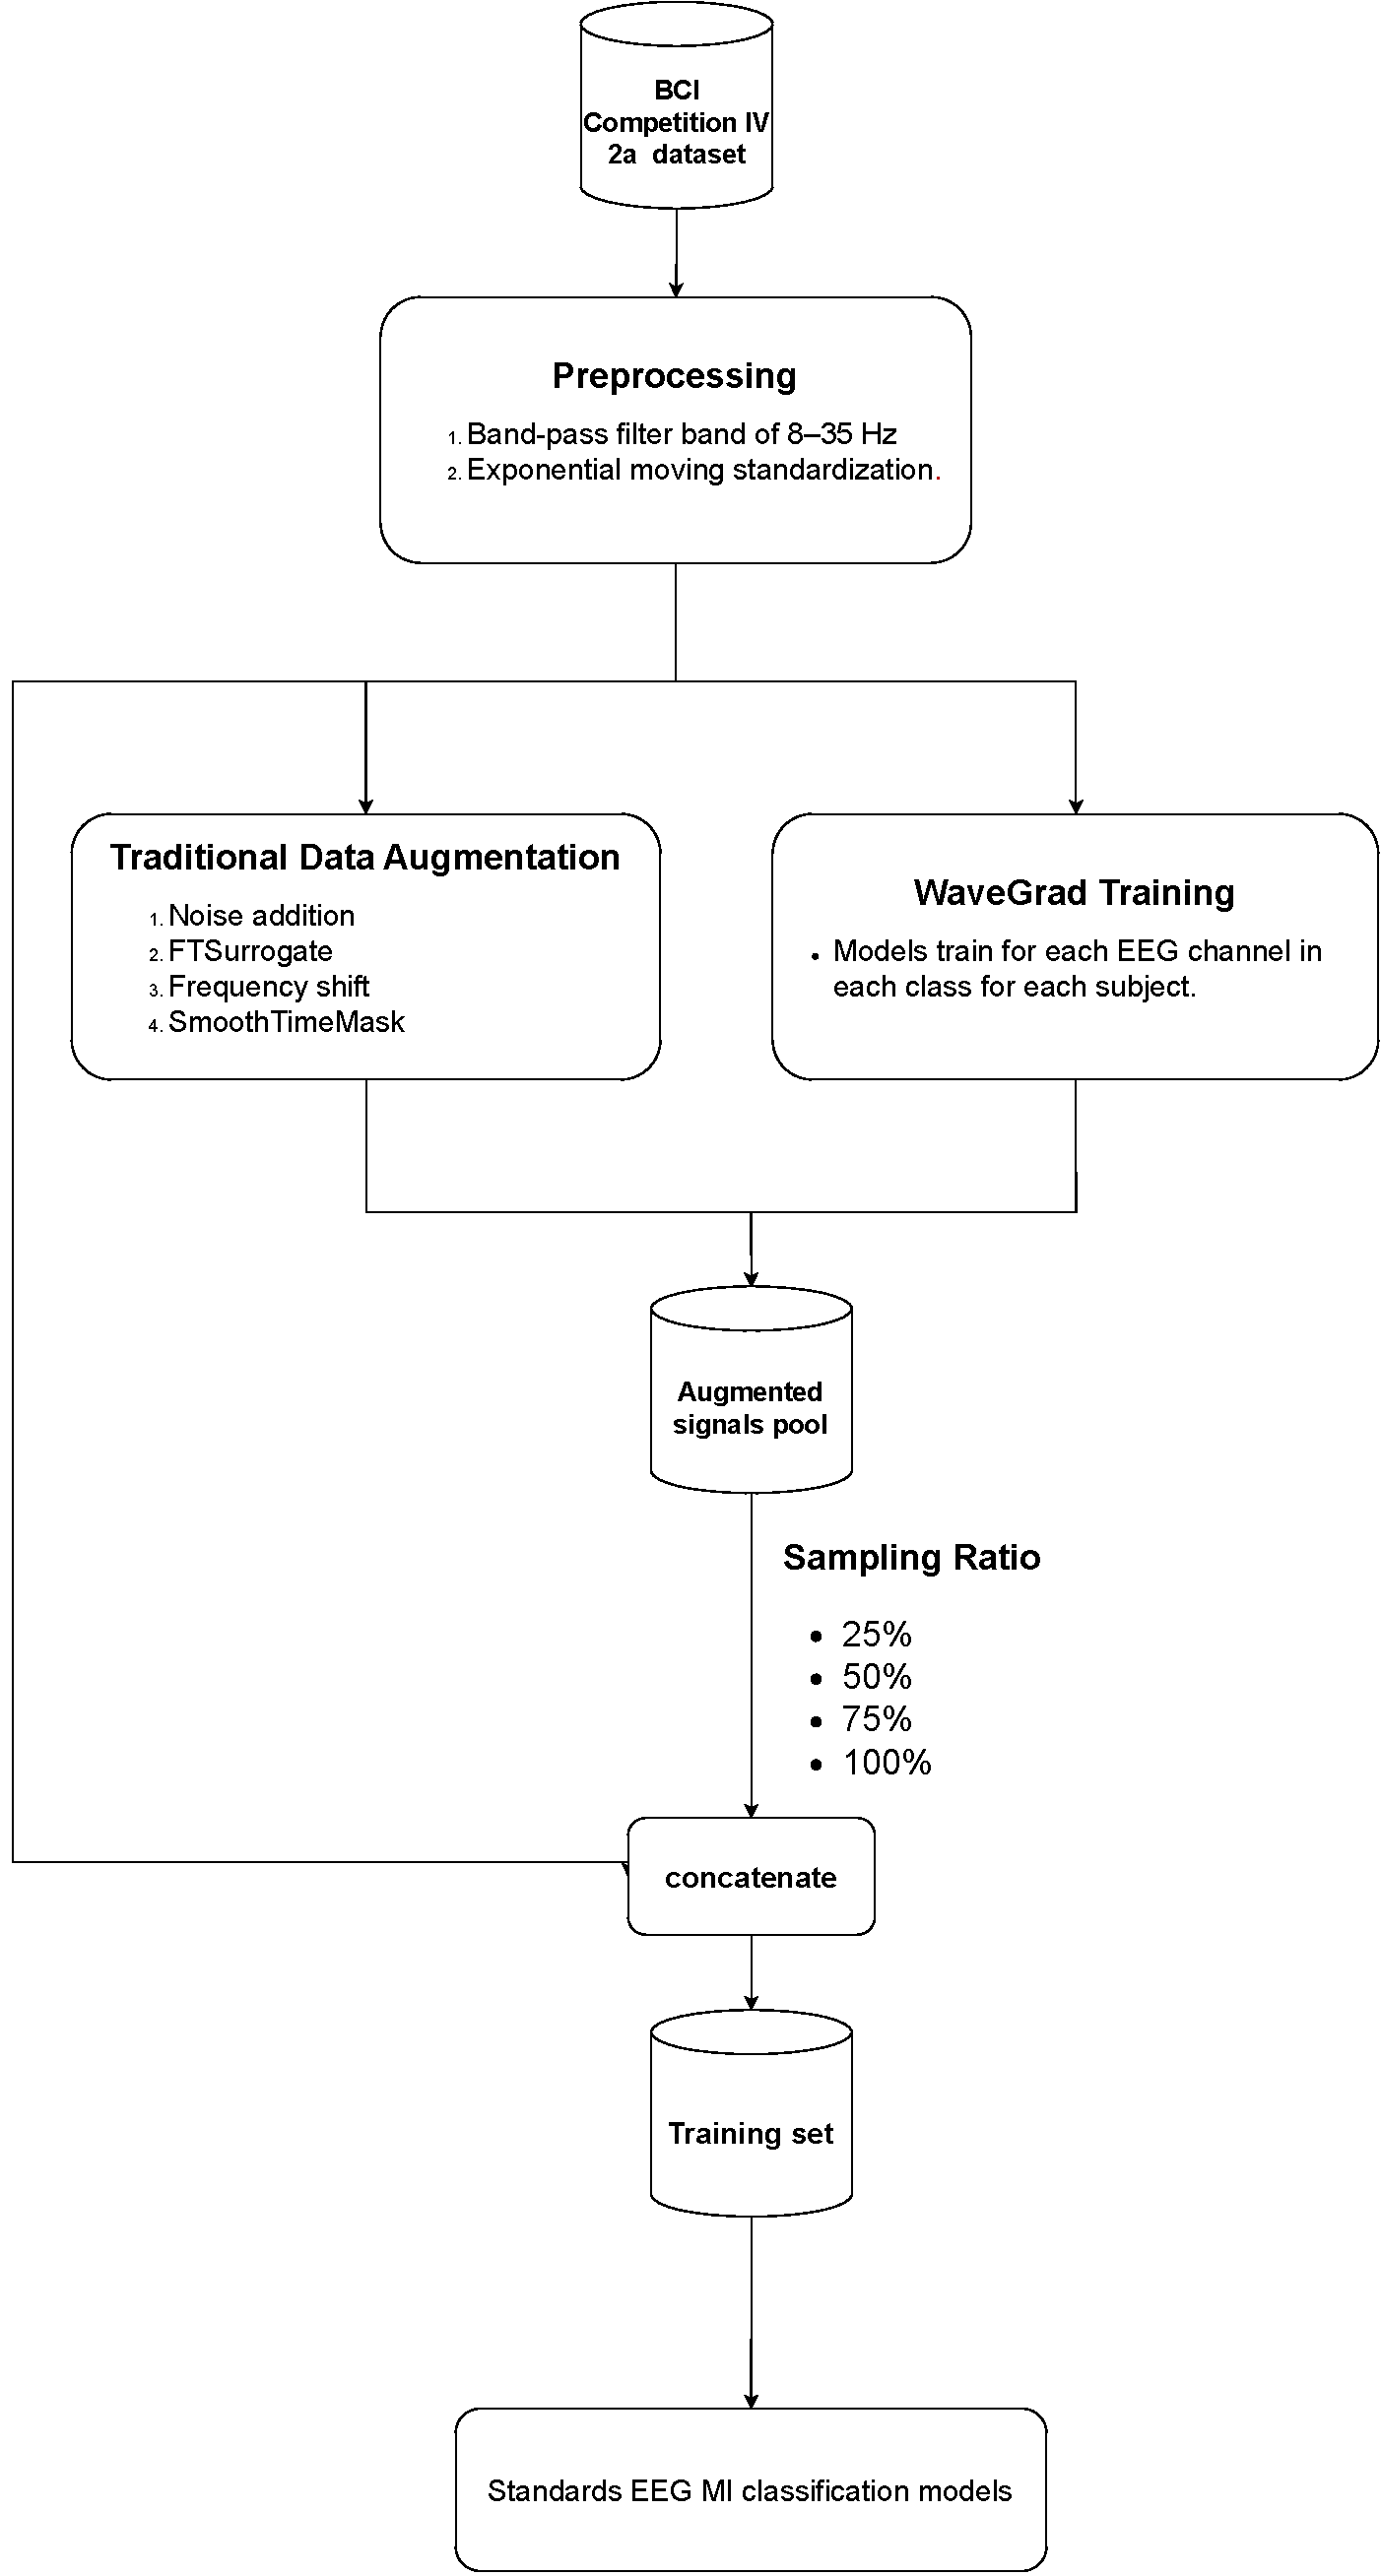
\includegraphics[width=0.6\textwidth]{fig/dyagram.pdf}
  \label{fig:System}
\end{figure}

\subsection{Datasets}
BCI Competition IV 2a \cite{brunner2008bci} was a collection of EEG data from 9 subjects who participated in a cue-based BCI paradigm involving four distinct motor imagery tasks: imagining movement of the left hand (class 1), the right hand (class 2), both feet (class 3) and the tongue (class 4).
Each subject completed the tasks in two distinct sessions on different days, with each session consisting of six runs separated by brief pauses, resulting in a total of 48 trials (12 for each of the four classes).
The data were captured while the participants sat in a comfortable armchair in front of a computer screen, and a fixation cross appeared at the start of each trial.
A cue consisting of an arrow pointing to the left, right, down, or up was used to prompt the subjects to perform the desired motor imagery task.
The subjects were instructed to perform the motor imagery task until the fixation cross disappeared from the screen without receiving any feedback.
Signals were sampled at 250 Hz and filtered between 0.5 Hz and 100 Hz using a 50 Hz notch filter to reduce line noise.
We used one section for training sets and another for test sets.

\subsection{Data Preprocessing}
EEG signal was filtered with a bandpass filter of 8 - 35 Hz followed by exponential moving standardization from \texttt{Braincode} library.

For exponential moving standardization, we computed the exponential moving mean $m_{t}$ at time $t$ as shown in equations (\ref{eq1}).
Then, we computed the exponential moving variance $v_{t}$ at time $t$ as shown in equation (\ref{eq2}).
Finally, we standardized the data point $x_{t}$ at time $t$ with $\alpha$ as 0.001 and $\epsilon$ as 0.0001 as shown in equation (\ref{eq3}).

\begin{eqnarray} 
m_{t} = \alpha \cdot \bar{x_{t}} + (1 - \alpha) \cdot m_{t-1}, \label{eq1}\\
v_{t} = \alpha\cdot (m_{t} - x_{t})^{2} + (1 - \alpha) \cdot v_{t-1} , \label{eq2} \\ 
x^{\prime}_{t} = \frac{(x_{t}-m_{t})}{\max(\sqrt{v_{t}},\epsilon), \label{eq3} }
\end{eqnarray}


\subsection{Data Augmentation}
Our objective was to assess the performance of each DA method with different ratios of augmented/synthetic data.
Five DA methods (\texttt{Noise Addition}, \texttt{FTSurrogate}, \texttt{Frequency Shift}, \texttt{SmoothTimeMask}, \texttt{WaveGrad}) and four ratios (25\%, 50\%, 75\%, 100\%) = 20 combinations (5 methods x 4 ratios) of the training set are to be created.
Here, ratios refer to the amount of augmented/synthetic data used.
For example, given a 25\% ratio, 25\% augmented data is randomly sampled and added to the original training set.
By comparing different ratios, we can better understand the impact of the size of augmentations on accuracy improvement.

Similar to previous works \cite{rommel2021cadda,mohsenvand2020contrastive,leeb2008bci,terzano2001atlas}, we used the subject-dependent scheme which augments data in subject level (i.e., each subject is treated separately) and channel level (i.e., each channel is treated independently).


\subsubsection{Noise Addition:}
\texttt{Noise Addition} entails the inclusion of diverse forms of noise, such as Gaussian, Poisson, and others, that possess varying parameters to the original EEG signal. 
The raw EEG signal was subjected to additive noise by incorporating a Gaussian distribution with a standard deviation of 0.1. 

\subsubsection{Fourier Transform Surrogates:}
\texttt{Fourier transform surrogates} are a type of data generated by randomizing the phases of temporal-spatial data.


\subsubsection{Frequency Shift:} The technique of \texttt{Frequency Shift} is characterized by the alteration of the frequency of the EEG signal by a specific amount.
We randomized the shift of the frequency by \textpm2 Hz.

\subsubsection{SmoothTimeMask:}
\texttt{SmoothTimeMask} involves applying a smooth window function to mask a continuous segment of the signal and optimizing it using gradient-based methods.
The signal was randomly masked with a range of 100 sample points.

\subsubsection{WaveGrad:}
It is first important that \texttt{WaveGrad} is originally a generative model, not a formal augmentation technique.
Thus, contrary to other DA methods, \texttt{WaveGrad} has to be trained before it can be used to generate a synthetic EEG signal.
The dataset consists of 9 subjects and four MI classes.
The EEG recording has 22 channels.
Thus, the total number of \texttt{WaveGrad} models was (9 subjects x 22 channels x 4 classes) = 792 models.
The training procedure and parameters were the same across all \texttt{WaveGrad} models.
The learning rate was set to 0.0001 and the diffusion steps to 1000.
% \textcolor{red}{talk more about what you add/modify}

\subsection{Evaluation}
First, it is important to evaluate the quality of the augmented/synthetic data.
A common way is through dimensionality reduction KL divergence.
The success of the diffusion method in comparison to other methods is demonstrated by the Kullback-Leibler (KL) divergence, which is used to measure the similarity between the training set (with and without augmentation) and the validation set.
We expect that high-quality augmented or synthetic data should exhibit similarity between the training set (with and without augmentation) and the validation set.

Second, once the quality of the augmented/synthetic data is quantified, we are now ready to quantify the usefulness of data augmentation techniques on actual EEG tasks.
We first selected five commonly used motor imagery classification models (EEGNet, ATCNet, EEG-ITNet, Deep ConvNet, and ShallowFBCSPNet) which would allow us to understand how the complexity of the model relates to data augmentation.
Here, note that we simply define the complexity based on the model's number of parameters.
Accuracy was then measured across all 21 combinations (5 DA methods x 4 sampling ratios + 1 baseline method without augmentation).
The details of each model were as follows:

\subsubsection{EEGNet}
%\textcolor{red}{intuition and parameters}
EEGNet is a single CNN architecture that can accurately classify EEG signals from different BCI paradigms while being as compact as possible.
The authors introduced the use of depthwise and separable convolutions to construct an EEG-specific model that encapsulates well-known EEG feature extraction concepts for BCI.
They compared EEGNet to current state-of-the-art approaches across four BCI paradigms and showed that EEGNet generalizes across paradigms and achieves comparably high performance when only limited training data is available across all tested paradigms.

\subsubsection{ATCNet}
%\textcolor{red}{intuition and parameters}
ATCNet was initially developed for predicting the onset of epileptic seizures using electroencephalogram (EEG) signals.
The ATCNet consists of two blocks: an attention-based temporal convolutional (ATC) block and a transformer-based classification (TC) block.
The ATC block is used to extract relevant features from the EEG signals, while the TC block is used to classify the extracted features into seizure and non-seizure classes.
The proposed model was evaluated using the BCI Competition IV-2a (BCI-2a) dataset.
The obtained accuracy ranged from 60.5\% to 89.5\%.

\subsubsection{EEG-ITNet}
EEG-ITNet uses inception modules and causal convolutions with dilation to extract rich spectral, spatial, and temporal information from multi-channel EEG signals with less complexity than other existing end-to-end architectures. 
The paper also provided a methodology for achieving intuitive visualization structures such as topographic maps.
The proposed EEG-ITNet model showed up to a 5.9\% improvement in classification accuracy compared to its competitors in different scenarios.

\subsubsection{Deep ConvNet}
The deep ConvNet had four convolution-max-pooling blocks, with a special first block designed to handle EEG input, followed by three standard convolution-max-pooling blocks and a dense softmax classification layer.
The authors found that recent advances in machine learning, including batch normalization and exponential linear units, together with a cropped training strategy, boosted the Deep ConvNets decoding performance, reaching at least as good performance as the widely used filter bank common spatial patterns (FBCSP) algorithm.

\subsubsection{ShallowFBCSPNet}
The shallow ConvNet is similar to the transformations of FBCSP.
Concretely, the first two layers of the shallow ConvNet perform a temporal convolution and a spatial filter, as in the deep ConvNet.
These steps are analogous to the bandpass and CSP spatial filter steps in FBCSP.

\section{Results}

\subsection{Kullback-Leibler divergence(KL divergence)}
To understand the quality of the generated data, we measured the similarity of the signal by the KL divergence process.
We measure the KL divergence by comparing of train set and test set, test set and train set with 25\% of data augmentation, test set and train set with 50\% of data augmentation, test set and train set with 75\% of data augmentation, test set and train set with 100\% of data augmentation in Table~\ref{tab:KL1}, and test set and data augmentation and train set and data augmentation in Table~\ref{tab:KL2}.
We randomized the augmentation data for this process 100 times and averaged the result.
Overall, our method increases similarity as the ratios of augmented data are increased.
When ratios are increased, the similarity for the SmoothTimeMask, Noise Addition, and FTSurrogate approaches that of the non-augmented data.
On the other hand, as the augmented data from frequency shift increases, the similarity declines.


\begin{table}[ht]
    \caption[The result of KL divergence]{\label{tab:KL1}The result of the study of KL divergence of raw EEG dataset and data augmentation from \texttt{WaveGrad}}.
    % \caption{\label{label}Table caption.}
    \begin{indented}
    \item[]\begin{tabular}{rccccc}
    \hline
    \multirow{2}{*}{Subject ID} & \multicolumn{5}{l}{test set vs train set with x\% of augmentation} \\ \cline{2-6} 
                                & 0\%         & 25\%        & 50\%        & 75\%        & 100\%      \\ \hline
    1                           & 2949.63     & 2757.15     & 2623.40     & 2525.57     & 2486.21    \\
    2                           & 1641.60     & 1887.98     & 2009.06     & 2118.49     & 2222.43    \\
    3                           & 2203.27     & 2298.26     & 2382.90     & 2416.10     & 2410.30    \\
    4                           & 2559.50     & 2390.33     & 2291.63     & 2240.40     & 2176.35    \\
    5                           & 2238.52     & 2215.49     & 2170.81     & 2146.55     & 2167.71    \\
    6                           & 1935.63     & 1999.40     & 2061.10     & 2067.91     & 2103.15    \\
    7                           & 2704.38     & 2564.74     & 2482.31     & 2424.12     & 2381.11    \\
    8                           & 3245.50     & 2946.14     & 2752.42     & 2628.08     & 2497.71    \\
    9                           & 2313.45     & 2290.44     & 2253.48     & 2231.11     & 2201.39   
    \end{tabular}
    \end{indented}
\end{table}

\begin{table}[]
    \caption[The result of KL divergence]{\label{tab:KL2}The result of the study of KL divergence of raw EEG dataset and data augmentation from \texttt{WaveGrad}}.
    \begin{indented}
    \item[]\begin{tabular}{rcc}
    \hline
    Subject ID & \multicolumn{1}{c}{Train set vs Augmentation} & \multicolumn{1}{c}{Test set vs Augmentation} \\ \hline
    1          & 1988.35                                        & 1582.51                                       \\
    2          & 2749.47                                        & 2970.01                                       \\
    3          & 2671.86                                        & 2800.51                                       \\
    4          & 1775.89                                        & 2193.34                                       \\
    5          & 2045.00                                        & 1870.57                                       \\
    6          & 2247.53                                        & 2069.20                                       \\
    7          & 2024.06                                        & 1808.16                                       \\
    8          & 1779.83                                        & 1398.65                                       \\
    9          & 2145.52                                        & 2123.10                                      
    \end{tabular}
    \end{indented}
\end{table}

\section{Discussion}
In this study, we demonstrated the implementation of the \texttt{WaveGrad}-based Diffusion Model as a DA for EEG MI datasets.
From the result, our method outperformed the other four traditional DA methods in the classification task.
Thus, for the discussion section, we focused mainly on our method.

\subsection{Key improvement}
The proposed methodology increased the variety of the train set, leading to an enhancement in the quality of the train set.
As shown in Figure~\ref{fig:KL-average}, the diffusion-based method created a new sample that is not a duplication of an existing one but shares the same characteristics.
Thus, the similarity between the train set with augmentation and the test set was increased. 
However, when performing augmentation with \texttt{Noise Addition}, \texttt{FTSurrogate}, and \texttt{SmoothTimeMask}, the similarity of the train set compared to the test set remains unchanged regardless of the augmentation.
This indicates that the augmented data does not share the characteristics of the dataset and it is obvious in the case of \texttt{SmoothTimeMask} and \texttt{Noise Addition}.
The same explanation could not be used with the case of the \texttt{Frequency shift} method.
While the similarity score was high when the augmentation was used, the classification performance was not improved at all. 
We believe the KL divergence might not be able to show the wrongness of this method.
Overall, our diffusion-based method improves the similarity of the test set and the train set (Figure~\ref{fig:KL-average}) and improves the classification performance (Table~\ref{table:AverageAccuracy}).

\begin{table}[ht!]
    \centering
    \caption{The Average accuracy improvement from our method on subject level.}
    \label{tab:AccuracySubject}
    \begin{tabular}{ccc}
        \hline
        Subject & Baseline Accuracy & \begin{math} \Delta \end{math} of \texttt{WaveGrad} \\
        \hline
        1        & 43.06             & 17.01             \\
        2        & 29.24             & 6.46              \\
        \textbf{3}        & \textbf{56.95}            & \textbf{15.36}             \\
        4        & 37.08             & 7.77              \\
        \textbf{5}        & \textbf{27.08}             & \textbf{4.13}              \\
        6        & 29.58             & 4.01              \\
        7        & 40.07             & 11.77             \\
        8        & 53.19             & 8.18              \\
        \textbf{9}        & \textbf{65.76}             & \textbf{2.59}              \\
        \hline
        \end{tabular}
\end{table}

\subsection{Subjects level}
We observed that the effectiveness of data augmentation was based on the quality of the dataset.
Table~\ref{tab:AccuracySubject} shows that subject 3 has a baseline accuracy of 56.95\% then improved by 15.46\% after the augmentation.
In contrast, subject 5's baseline accuracy was measured to be 28.08\% in the study and the improvement after the augmentation was small with 4.13\%. 
In addition, the improvement gained with the augmentation in subject 9's case is small even though the baseline accuracy is the highest out of all subjects.
This could be due to the limitation of the classification model. 


\begin{table}[ht!]
    \centering
    \caption{The Average accuracy improvement from our method on DA size level.}
    \label{table: The Average accuracy improvement from our method on DA size level}
    \begin{tabular}{ccccc}
        \hline
        Baseline Accuracy & DA size & \texttt{WaveGrad} & \begin{math} \sigma \end{math} & \begin{math} \Delta \end{math} \\
        \hline
        42.45             & 25\%    & 51.15    & 17.61                        & 8.71              \\
                          & 50\%    & 50.56    & 17.38                        & 8.11              \\
                          & 75\%    & 51.64    & 17.24                        & 9.19              \\
                          & 100\%   & 50.78    & 17.72                        & 8.33              \\
        \hline
        \end{tabular}
\end{table}
        
\subsection{Size of DA}
The effect of the size of DA on the classification performance was not a direct variation.
Table~\ref{table: The Average accuracy improvement from our method on DA size level} presented the average accuracy improvement achieved by our method on the DA size level.
The limitations of the dataset used to train the \texttt{WaveGrad} method have impacted its capacity to produce signals with greater valence.
The observed limitation might account for the non-linear relationship between the size of the data augmentation and the corresponding increase in accuracy. 
The result suggested that increasing the number of samples may not necessarily lead to a significant enhancement in accuracy, particularly if the additional samples fail to encompass the complete spectrum of potential signal fluctuations.

However, despite this limitation, the \texttt{WaveGrad} method still outperformed the baseline accuracy on all levels of data augmentation, with the highest improvement achieved at a DA size of 75\%. 
This finding suggested that even with a limited dataset, data augmentation techniques such as \texttt{WaveGrad} can still be effective in improving the accuracy of motor imagery classification.

It was worth noting that the results presented in the table were based on a single dataset, and the effectiveness of the \texttt{WaveGrad} method varies with other datasets or signal processing tasks. 
Future studies should investigate the generalizability of the \texttt{WaveGrad} method and explore its potential for improving accuracy in other EEG-based classification tasks.

The study concluded that although the \texttt{WaveGrad} method's capacity to produce signals with higher valence is affected by the restricted dataset used for its training, the outcomes presented in the table indicated that the method can enhance the precision of the motor imagery classification task using EEG signals. 
Additional investigation was required to establish the applicability of the \texttt{WaveGrad} approach to alternative datasets and signal processing assignments.


\begin{table}[ht!]
    \centering
    \caption{The Average accuracy improvement from our method.}
    \label{table: The Average accuracy improvement from our method}
    \begin{tabular}{ccccc}
        \hline
        Model           & Baseline Accuracy & \texttt{WaveGrad} & \begin{math} \sigma \end{math} & \begin{math} \Delta \end{math} \\
        \hline
        ATCNet          & 47.68             & 53.63    & 18.45                        & 5.94  \\
        Deep ConvNet    & 32.60             & 52.93    & 18.49                        & 20.33 \\
        EEGITNet        & 46.84             & 54.96    & 16.76                        & 8.12  \\
        EEGNet          & 34.18             & 37.04    & 8.00                         & 2.85  \\
        ShallowFBCSPNet & 50.93             & 56.62    & 15.85                        & 5.69 \\
        \hline
        \end{tabular}
\end{table}

\subsection{Complexity of models}
In a low-complexity model, our method improves accuracy more than the model with high-complexity as shown Table~\ref{table: The Average accuracy improvement from our method}.
We suspected that the model with high complexity might be overfitting to the train set.
As a result, to assess the effect of diffusion-based data augmentation of the high-complexity model, we might need to change the dataset or task that suited the complexity.

\subsection{Limitation}
First, the proposed data augmentation method was developed based on a limited dataset, specifically the BCI competition IV dataset 2a. 
While the method showed promising results on this dataset, its effectiveness might be limited by the size and quality of the dataset used for its development. 
Future work could involve evaluating the generalizability of the method on other EEG MI datasets to improve its confidence in wider usage scenarios.
Second, the proposed data augmentation method was developed specifically for the EEG MI task. 
It might not necessarily generalize well to other EEG-based tasks. 
Future work could involve evaluating the method on other EEG signal tasks, such as P300 and SSEVP, to assess its robustness and adaptability across different EEG-based applications.



\section{Conclusion}
In this study, we investigated the effectiveness of data augmentation techniques in improving the accuracy of standard EEG MI classification models. 
We used five standard EEG MI classification models to classify EEG signals into left and right hand movements. 
We evaluated the performance of data augmentation techniques by comparing them with the baseline model, which was trained without any data augmentation. 
For the data augmentation techniques, we used \texttt{WaveGrad}, \texttt{Noise Addition}, \texttt{Frequency Shift}, \texttt{Fourier transform surrogates}, and \texttt{SmoothTimeMask}.

Our results showed that data augmentation techniques improved the performance of standard EEG MI classification models, with \texttt{WaveGrad} being the most effective technique. 
The accuracy of the baseline model was 42.45\%, while the accuracy of the model trained with 75\% synthetic data generated by \texttt{WaveGrad} was 51.64\%. 
The other data augmentation techniques also improved the performance of the models, with \texttt{Noise Addition} and \texttt{Frequency Shift} being the least effective techniques.



\section*{References}
\bibliographystyle{iopart-num}
\bibliography{references}






\end{document}

